%% packages
\documentclass{article}
\usepackage[a4paper, left=2.0cm, right=2.0cm, top=3.5cm]{geometry}
\usepackage[ngerman]{babel}
\usepackage{graphicx}
\usepackage{multicol}
\usepackage{amssymb}
\usepackage{titlesec}
\usepackage{wrapfig}
\usepackage{blindtext}
\usepackage{lipsum}
\usepackage{caption}
\usepackage{listings}
\usepackage{fancyhdr}
\usepackage{nopageno}
\usepackage{authblk}
\usepackage{amsmath} % tons of math stuff
\usepackage{mathtools} % e.g. alignment within matrix
%\usepackage{bm} % provides shorthand for bold in math mode
\usepackage{dsfont} % \mathds makes double stroke digits
\usepackage{esdiff} % provides \diff
%\usepackage[ISO]{diffcoeff}
\usepackage{xcolor}
\usepackage{csquotes} % e.g. provides \enquote
\usepackage[separate-uncertainty=true]{siunitx} % units
\usepackage{xcolor} % colored text
\usepackage{csvsimple}
\usepackage{subcaption}
\usepackage{physics}
\usepackage{hyperref}
\usepackage{nameref}
\hypersetup{colorlinks=true, linkcolor=black, pdfhighlight={/N}}
\usepackage{tcolorbox}
\usepackage{amsthm}
\usepackage{float}
\usepackage{enumitem}
\usepackage{booktabs}

% \sisetup{
%   scientific-notation = auto,  % Automatically use scientific notation for large/small numbers
%   output-exponent-marker = \text{e}  % (optional) for formatting the exponent symbol
% }

%\fancyhf[]{}

%% custom stuff
% own units
\DeclareSIUnit \VSS {\ensuremath{V_\mathrm{SS}}}
\DeclareSIUnit \VS {\ensuremath{V_\mathrm{S}}}
\DeclareSIUnit \Veff {\ensuremath{V_\mathrm{eff}}}
\DeclareSIUnit \Vpp {\ensuremath{V_\mathrm{pp}}}
\DeclareSIUnit \Vp {\ensuremath{V_\mathrm{p}}}
\DeclareSIUnit \VRMS {\ensuremath{V_\mathrm{RMS}}}
\DeclareSIUnit \ASS {\ensuremath{A_\mathrm{SS}}}
\DeclareSIUnit \AS {\ensuremath{A_\mathrm{S}}}
\DeclareSIUnit \Aeff {\ensuremath{A_\mathrm{eff}}}
\DeclareSIUnit \App {\ensuremath{A_\mathrm{pp}}}
\DeclareSIUnit \Ap {\ensuremath{A_\mathrm{p}}}
\DeclareSIUnit \ARMS {\ensuremath{A_\mathrm{RMS}}}

% change subsection numbering to capital letters
\newcommand{\subsectionAlph}{ \renewcommand{\thesubsection}{\arabic{section}.\Alph{subsection}} }
% change subsection numbering to lowercase letters
\newcommand{\subsectionalph}{ \renewcommand{\thesubsection}{\arabic{section}.\alph{subsection}} }
% change subsubsection numbering to lowercase letters
\newcommand{\subsubsectionalph}{ \renewcommand{\thesubsubsection}{\arabic{section}.\arabic{subsection}.\alph{subsubsection}} }
% own fig. that works with multicols
\newenvironment{Figure}
  {\par\medskip\noindent\minipage{\linewidth}}
  {\endminipage\par\medskip}
\newcommand*{\inputPath}{./plot} % prepend this command to the argument of all input commands
\graphicspath{ {./images/}{./figure/}{../plot/}{../../plot/}{../../latex/assets/}{./assets/} }
% own enviroment for definitions
\newenvironment{definition}[1]
{\begin{quote} \noindent \textbf{\textit{#1\ifx&#1& \else : \fi}} \itshape}
{\end{quote}}



% own commands
% \newcommand{\rarr}{$\to\,$} %A$\,\to\,$B
\newcommand{\defc}{black}
\newcommand{\colorT}[2][blue]{\color{#1}{#2}\color{\defc}}
\newcommand{\redq}{\color{red}(?)\color{\defc}}
\newcommand{\question}[1]{\colorT[purple]{\textbf{(#1)}}}
\newcommand{\todo}[1]{\colorT[red]{\textbf{(#1)}}}
\newcommand{\mr}{\mathrm}


%% preparation


%dachte wir können hier durchführung und gleich Auswertung der einzelnen Versuchsaufgaben schreiben und im Fazit ein gesamtfazit

%\displaystyle \lim_{x \to \infty}

\begin{document}
    \title{Elektronikpraktikum \\ \textbf{Versuch 2: Diodenkennlinien}}
    \author[1]{Carlos Pascua \thanks{s87cpasc@uni-bonn.de}}
    \author[1]{Anna Maróti\thanks{s32amaro@uni-bonn.de}}
    \author[1]{Cornelius Heiming\thanks{s64cheim@uni-bonn.de}}
    \affil[1]{Uni Bonn}
    %\date{\today}
	\pagenumbering{gobble}
    \begin{titlepage}
     \maketitle   
    \end{titlepage}
        
\tableofcontents
\newpage
\pagenumbering{arabic}

\pagestyle{fancy}
\fancyhead[R]{\thepage}
\fancyhead[L]{\leftmark}

\section{Theorie}

\subsection*{Einführung}

In diesem Versuch wird 
\section{Voraufgaben}

\begin{enumerate}[label=\textbf{(\Alph*)}]
    \item \textbf{Was bestimmt die Dicke der Grenzschicht bei einem p-n-Halbleiter?}
    \\ Wenn man bei einer p-n Halbleiter eine Spannung anlegt, werden es Elektronen und Löcher diffundieren 
    und bleiben im Halbleiter Donatorionen bzw. Akzeptaronionen übrig, die 
    zusammen ein elektrisches Feld bilden. Diese wird immer größer, bis die genauso groß, wie die 
    Spannung, die von der Difussion von Löcher und Elektronen ist. 
    \item \textbf{Wie ändert sich die Kapazität einer Diode im Sperrfall mit der angelegten Spannung?}
    \\ Im Sperrbetrieb bildet sich in der Halbleiterdiode eine Raumladungszone mit gespeicherten
     Ladungen. Diese Zone wirkt wie ein Plattenkondensator mit der Kapazität
      \( C = \varepsilon_0 \varepsilon_r A / d \), wobei \( d \) dem effektiven Ladungsträgerabstand entspricht. Wird die Sperrspannung erhöht, vergrößert sich \( d \), und die Kapazität nimmt entsprechend ab.
 
    \item \textbf{Skizzieren Sie den Kennlinienverlauf $I = f(U)$ der Zweipole aus Abb. 1 (R = \SI{100}{\ohm}; D = Diode). Erläutern Sie bei c) und d) den Einfluss der Widerstände.}
    \\ Bei Schaltung (c) begrenzt der in Reihe geschaltete Widerstand den Stromfluss, sobald die Durchlassspannung der Diode erreicht ist. In Schaltung (d) hingegen bewirkt der parallel geschaltete Widerstand, dass bereits bei kleinen Eingangsspannungen ein Teil des Stroms über ihn abfließen kann.
 
    \item \textbf{Skizzieren Sie den zeitlichen Verlauf der Ausgangsspannungen der Schaltungen in Abb. ??, wenn die Eingangsspannung eine weit über der Durchlassspannung der Dioden liegende Sinusspannung ist.}
    \\ 
    \item \textbf{Wie muss $C$ dimensioniert sein, um die Welligkeit der Spannung über $R$ möglichst klein zu halten?}
    \\ Um die Welligkeit der Ausgangsspannung möglichst gering zu halten, sollte der Kondensator die Spannungsminima überbrücken können. Dazu muss die Zeitkonstante \( \tau = RC \) in der Größenordnung des Abstands \( T \) zwischen zwei Spannungsmaxima liegen. Daraus folgt näherungsweise \( C \sim \tau / R \).

    \item \textbf{Wie würden Sie Strom- und Spannungsmessgerät zur Messung der Kennlinie in Durchlassrichtung und in Sperrrichtung anordnen? Berücksichtigen Sie die Innenwiderstände der beiden Geräte.}
    \\In Durchlassrichtung sollte spannungsrichtig gemessen werden, da der Spannungsabfall über der Diode gering, der Strom jedoch vergleichsweise groß ist. In Sperrrichtung empfiehlt sich eine stromrichtige Messung, da hier hohe Spannungen bei sehr kleinen Strömen auftreten.

    \item \textbf{Wie kann man sich eine zu einem Strom proportionale Spannung herstellen?}
    \\ Eine zu einem Strom proportionale Spannung kann mithilfe eines ohmschen Widerstands erzeugt werden, da gemäß dem Ohm’schen Gesetz \( U = R \cdot I \) gilt.

    \item \textbf{Für Abb. 5: Berechnen Sie größenordnungsmäßig die größte Kapazität, die benutzt werden darf, ohne die Grenzwerte der Si-Diode zu überschreiten.}
    \\ Die maximale Kapazität ergibt sich aus dem Zusammenhang \( C = \frac{Q}{U} = \frac{I \cdot \Delta t}{\Delta U} \).  
    Setzt man die Werte \( I_\text{max} = \SI{1000}{\milli\ampere} \), \( \Delta t = \SI{100}{\micro\second} \) und \( \Delta U = \SI{1}{\volt} \) ein, so ergibt sich:
    \[
    C_\text{max} = \frac{I_\text{max} \cdot \Delta t}{\Delta U} = \frac{\SI{1000}{\milli\ampere} \cdot \SI{100}{\micro\second}}{\SI{1}{\volt}} = \SI{100}{\micro\farad}
    \]
    
    \item \textbf{Skizzieren Sie den zeitlichen Verlauf der Spannung am Ausgang der Schaltungen in Abb. 2.9.}
    
    \item \textbf{Skizzieren Sie die Lastabhängigkeit der Spannung $U'$ in Abb. 8 a). Geben Sie die Formel an, aus der sich $U'$ in Abhängigkeit von $U_0$, $R$ und $R_L$ berechnen lässt. Was sind die Extremwerte für $U'$ und $I$?}
    \\ Da es sich um eine Spannungsteilerschaltung handelt, gilt:
    \[
    U' = U_0 \cdot \frac{R_L}{R_L + R}
    \]
    Für \( R_L \to 0 \) folgt \( U' \to 0 \) und der Strom \( I \to \frac{U_0}{R} \).  
    Für \( R_L \to \infty \) ergibt sich \( U' \to U_0 \) und \( I \to 0 \).  
    Der qualitative Verlauf der Ausgangsspannung in Abhängigkeit von \( R_L \) ist in Abbildung dargestellt.
    
    \item \textbf{Innerhalb welches Wertebereichs muss bei dieser Dimensionierung der Arbeitswiderstand $R$ liegen, damit die Ausgangsspannung $U'$ bei der Zenerspannung von \SI{8.2}{\volt} stabilisiert wird?}
   \\ Damit die Zenerdiode bei einer Zenerspannung von \( U_Z = \SI{8.2}{\volt} \) zuverlässig stabilisiert, muss der Vorwiderstand \( R \) innerhalb eines bestimmten Wertebereichs liegen:

Für den Fall \( R_L = \infty \) fließt der gesamte Strom durch die Diode. Um den maximal zulässigen Zenerstrom \( I_{Z,\text{max}} = \SI{100}{\milli\ampere} \) nicht zu überschreiten, ergibt sich die untere Grenze für \( R \) aus dem Ohm’schen Gesetz:
\[
R > \frac{U_{0,\text{max}} - U_Z}{I_{Z,\text{max}}} = \frac{\SI{22}{\volt} - \SI{8.2}{\volt}}{\SI{100}{\milli\ampere}} = \SI{138}{\ohm}
\]

Für den Fall minimaler Eingangsspannung \( U_{0,\text{min}} = \SI{16}{\volt} \) und einer Last von \( R_L = \SI{200}{\ohm} \), soll mindestens \( I_{Z,\text{min}} = \SI{2}{\milli\ampere} \) durch die Diode fließen. Dann ergibt sich:
\[
R < \frac{U_{0,\text{min}} - U_Z}{I_{Z,\text{min}} + \frac{U_Z}{R_L}} = \frac{\SI{16}{\volt} - \SI{8.2}{\volt}}{\SI{2}{\milli\ampere} + \frac{\SI{8.2}{\volt}}{\SI{200}{\ohm}}} \approx \SI{181.4}{\ohm}
\]

Somit liegt der zulässige Bereich für den Vorwiderstand \( R \) zwischen etwa \SI{138}{\ohm} und \SI{181}{\ohm}.

\end{enumerate}



\section{Stabilisierung mit Zenerdiode}

\begin{figure}[H]
             \centering
             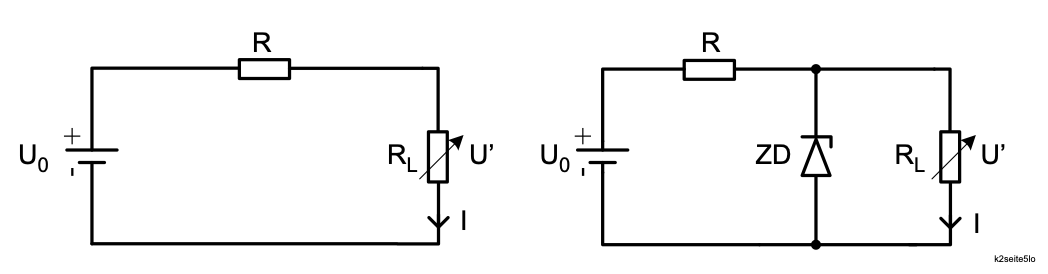
\includegraphics[width=0.8\textwidth]{Versuch0/figs/fig2_11.png}
             \caption{Spannungsstabilisierung ohne/mit Zenerdiode \cite{anleitung}}
             \label{fig:Zenerdiode}
         \end{figure}

Dann wurde das Verhalten von Spannungsstabilisierung durch eine Zenerdiode weiter untersucht. Hierzu wurde die Schaltung 
\autoref{fig:Zenerdiode} aufgebaut, um eine Einweggleichrichter zu erzeugen. Die Spannung wurde zusätzlich mit
 einem Kondensator mit $C= \SI{22}{\micro \farad}$ geglättet. Dieses hat dazu beigetragen, dass statt der positiven 
 Halbwelle des Sinussignals, die Spannung langsamer abnimmt und es einen sägezahnförmigen Verlauf ergibt, wie
  in \autoref{AufgabeEinwegrichter} ?? schon betrachtet und erklärt.
Der Lastwiderstand $R= \SI{150}{\ohm}$ wurde anhand der Voraufgabe K gewählt, da diese im errechneten Wertebereich 
liegt(\autoref{voraufgabe K}). Dann wurden die aufgebauten Schaltungen untersucht, indem die Spannung und Stromstärke
 am Lastwiderstand $R_L$ gemessen wurden, indem mit einem Potentiometer der Lastwiderstand verändert wurde. Beim Aufbau
  ohne der Zenerdiode wurde zusätzlich die Brummspannung aufgenommen, indem vom Oszillographen der peakpeak-Spannung abgelesen wurde.
   Die angegebenen Messunsicherheiten aus \autoref{tab:Lastwiderstand_mit_Fehlern} und \autoref{tab:Stabilisierung_mit_Fehlern} wurden
    basierend auf die Genauigkeit des Multimeters bestimmt. \cite{Digitalmultimeter}

??
https://die-kettwiger.jimdofree.com/braun-design/messen-technik/multimeter-digital/m2005/


\begin{table}[h!]
\centering
\begin{tabular}{|c|c|c|c|c|c|}
\hline
\textbf{$U'$ [V]} & \textbf{$\Delta U'$ [V]} & \textbf{$I$ [$m$A]} & \textbf{$\Delta I$ [$m$A]} & \textbf{$V_\text{Brumm}$ [V]} & \textbf{$\Delta V_\text{Brumm}$ [V]} \\
\hline
0.022 & 0.001 & 44.3 & 0.5 & 1.2 & 0.1 \\
1.642 & 0.009 & 39.9 & 0.4 & 4.4 & 0.1 \\
5.120 & 0.026 & 31.9 & 0.3 & 8.8 & 0.1 \\
7.050 & 0.036 & 28.1 & 0.3 & 10.3 & 0.1 \\
9.060 & 0.046 & 24.3 & 0.3 & 10.6 & 0.1 \\
11.390 & 0.058 & 20.1 & 0.2 & 10.2 & 0.1 \\
13.980 & 0.071 & 15.4 & 0.2 & 9.2 & 0.1 \\
16.920 & 0.086 & 10.4 & 0.1 & 6.8 & 0.1 \\
19.940 & 0.101 & 5.3 & 0.1 & 4.0 & 0.1 \\
21.940 & 0.111 & 2.2 & 0.0 & 2.2 & 0.1 \\
\hline
\end{tabular}
\caption{Messwerte ohne Stabilisierung mit Lastwiderstand (aktualisierte Unsicherheiten)}
\label{tab:Lastwiderstand_mit_Fehlern}
\end{table}



\begin{table}[h!]
\centering
\begin{tabular}{|c|c|c|c|}
\hline
\textbf{$U'$ [V]} & \textbf{$\Delta U'$ [V]} & \textbf{$I$ [$m$A]} & \textbf{$\Delta I$ [$m$A]} \\
\hline
0.021 & 0.001 & 44.0 & 0.5 \\
2.456 & 0.013 & 37.6 & 0.4 \\
4.690 & 0.024 & 30.8 & 0.3 \\
5.200 & 0.027 & 27.9 & 0.3 \\
6.170 & 0.032 & 21.7 & 0.2 \\
6.980 & 0.036 & 16.0 & 0.2 \\
7.320 & 0.038 & 13.5 & 0.1 \\
7.980 & 0.041 & 7.9 & 0.1 \\
8.250 & 0.042 & 4.8 & 0.1 \\
8.410 & 0.043 & 0.8 & 0.0 \\
\hline
\end{tabular}
\caption{Messwerte mit Stabilisierung und Lastwiderstand (aktualisierte Unsicherheiten)}
\label{tab:Stabilisierung_mit_Fehlern}
\end{table}


\begin{figure}[H]
             \centering
             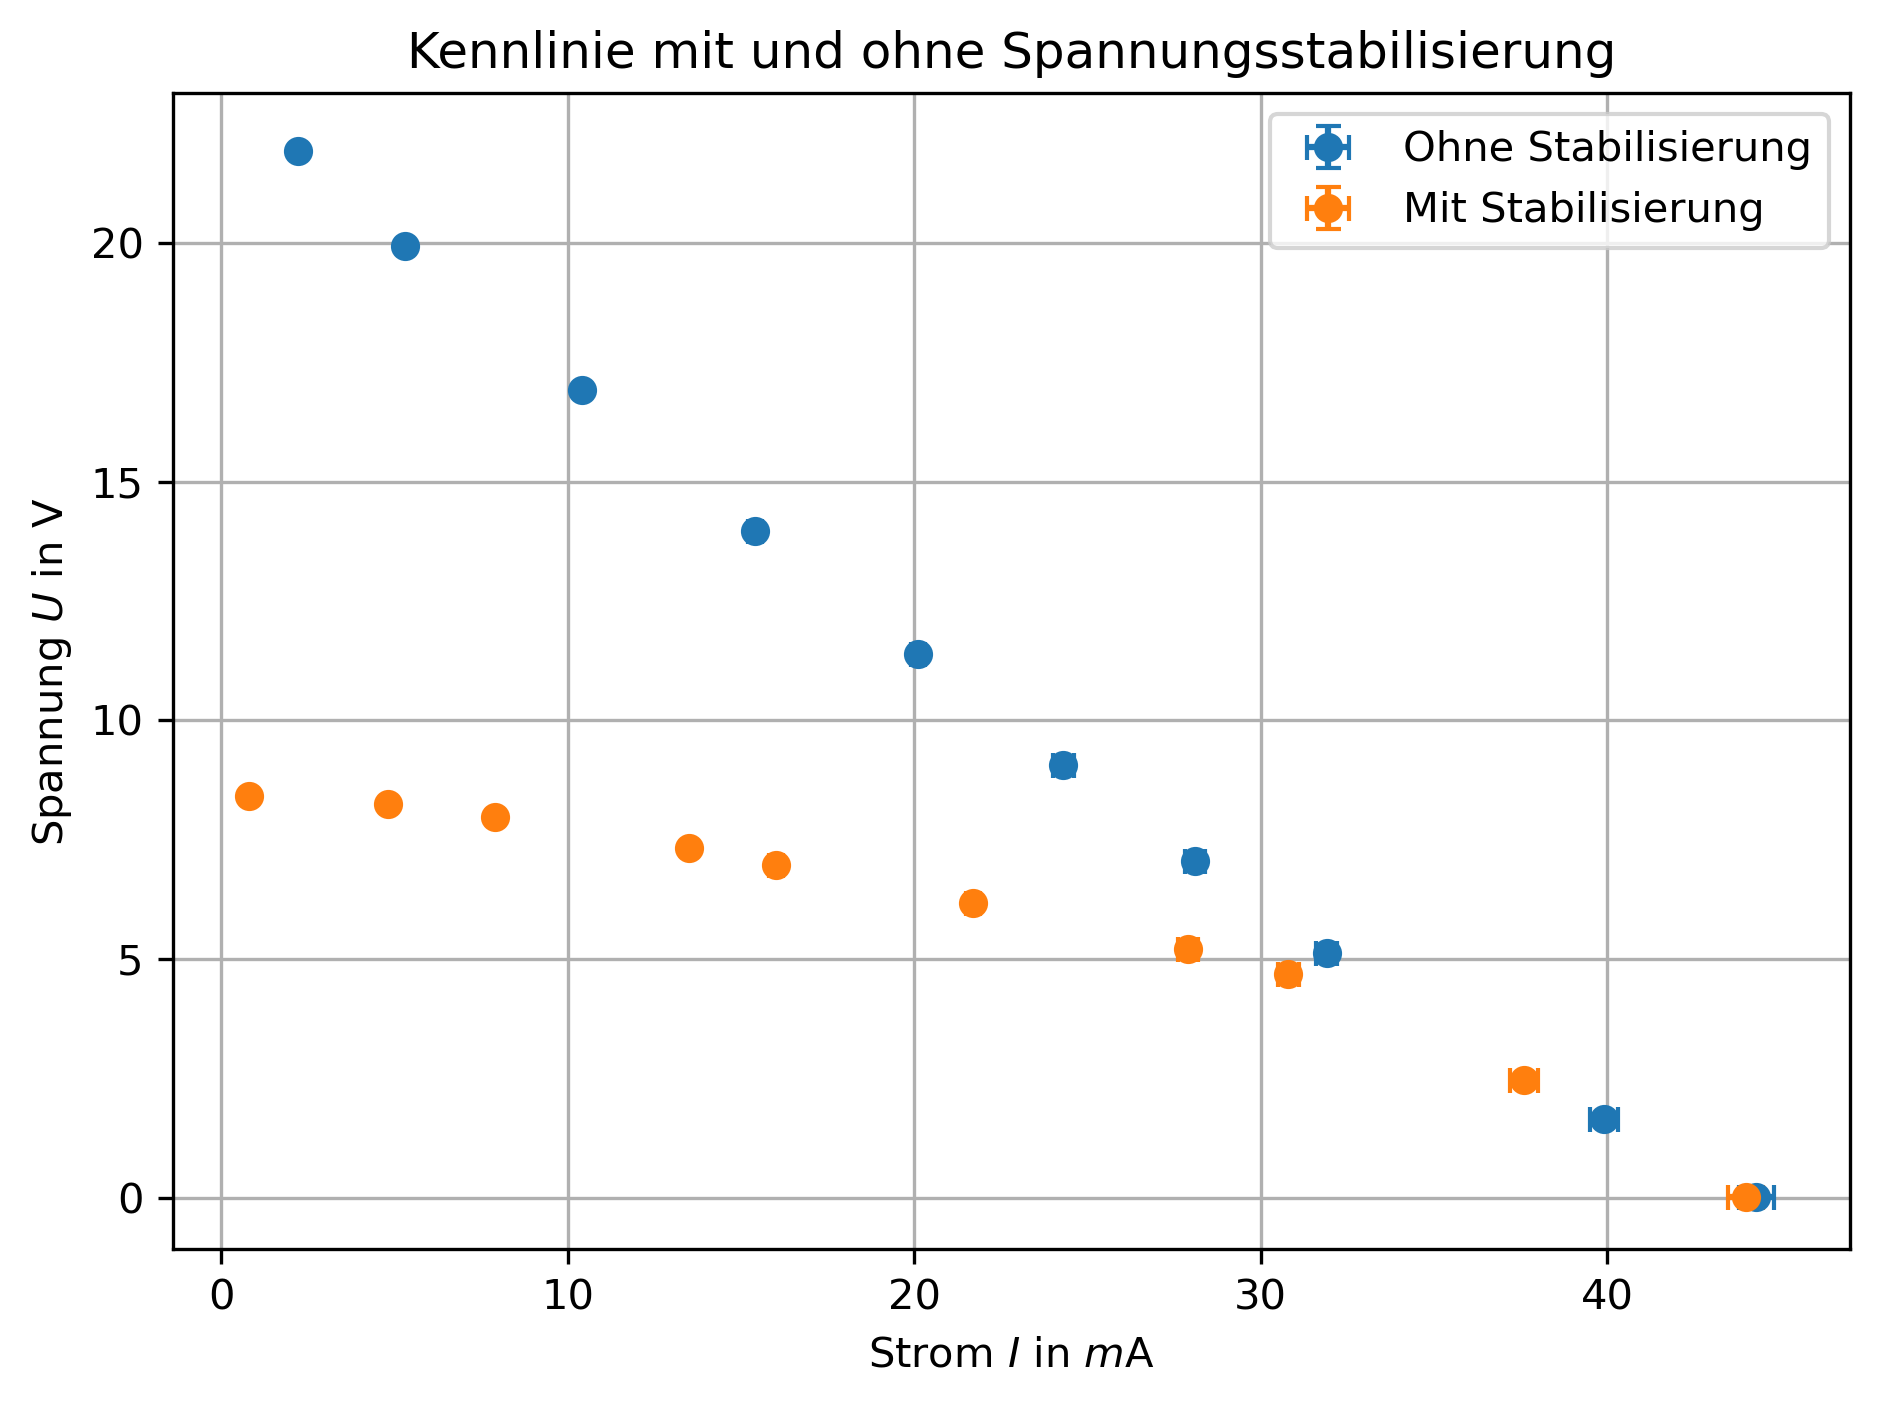
\includegraphics[width=0.8\textwidth]{Versuch0/figs/2.5.png}
             \caption{Kennlinie mit und ohne Stabilisierung einer Zenerdiode. Unsicherheiten sind eingetragen, treten im Graphen nicht auf, wenn sie zu klein zum Abbilden sind.}
             \label{fig:Stabilisierung}
         \end{figure}
         
         
Am \autoref{fig:Stabilisierung} kann man nun die Kennlinien von Widerständen mit und ohne Stabilisierung gut erkennen. Zunächst gibt es einen linearen Zusammenhang zwischen $U$ und $I$ ohne Stabilisierung. Dieses war aus dem ohmschen Gesetz $U= R \cdot I$ zu erwarten und bestätigt die richtige Aufnahme der Daten. Mit der Zenerdiode, kann man erkennen, dass die Spannung für kleine Ströme stabilisiert. Dieses erkennt man daran, dass es einen Knick im Graphen gibt und die Spannung im Intervall $[\SI{0}{\milli \ampere}, \SI{30}{\milli \ampere}]$ zwischen $\SI{8.5}{\volt}$ und $\SI{5}{\volt}$ bleibt. Diese Stabilisierung wurde durch die Zenerdiode erreicht. Sie wurde in Sperrrichtung betrieben und lass nur kleinere vom Widerstand unabhängige Ströme hindurch, weshalb der Betrag der Spannung über einen Bereich nur wenig Veränderung aufweist. Nach dem Ohmschen Gesetz kann nun bestimmt werden, aber welcher Lastspannung die Stabilisierung erfolgt. Hierzu wird aus dem Graphen der Knickpunkt bei $U' = \SI{5\pm 1}{\volt}$ und $I = \SI{30 \pm 2}{\milli \ampere}$ verwendet.

\begin{align}
    R_L &= \frac{U'}{I} = \frac{\SI{5}{\volt}}{\SI{30}{\milli \ampere}} \approx \SI{166.7}{\ohm} \\
    \Delta R_L &= \sqrt{\left( \frac{\Delta U'}{I}\right)^2 + \left( \frac{\Delta I \cdot U'}{I^2}\right)^2} \approx \SI{35.1}{\ohm}
\end{align}


Die Stabilisierung wirkt also ab einem Lastwiderstand von $R_L = \SI{166.7\pm 35.1}{\ohm}$. In der Voraufgabe K wurde der Arbeitswiderstand bestimmt, damit die Stabilisierung für den Lastwiderstand von $R_L > \SI{200}{\ohm}$ erfolgt. Der berechnete Wert schließt diesen mit seiner Unsicherheit ein. Ohne der Betrachtung der Unsicherheit gibt es eine totale Abweichung von etwa $17\%$. Diese größere Abweichung entstand, da man aus dem Graphen schwierig einen genauen Knickpunkt ablesen konnte, weshalb die Unsicherheiten auch so groß gewählt wurden. Außerdem kann es bei der Messung auch durch weitere Messunsicherheiten gekommen sein, da in der Realität systematische Fehler der Geräte und Schaltungen eine Rolle spielen.


\begin{figure}[h!]
    \centering
    % Erste Reihe
    \begin{subfigure}[b]{0.45\textwidth}
        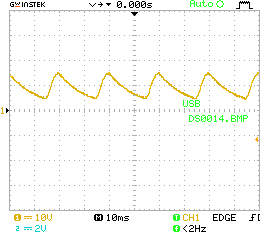
\includegraphics[width=\textwidth]{Versuch0/MesswerteVersuch2/DS0014.png}
    \end{subfigure}
    \hfill
    \begin{subfigure}[b]{0.45\textwidth}
        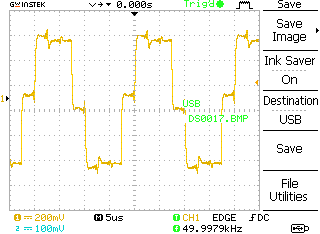
\includegraphics[width=\textwidth]{Versuch0/MesswerteVersuch2/DS0017.png}
      
    \end{subfigure}

    \vspace{0.5cm} % Abstand zwischen den Zeilen

    % Zweite Reihe
    \begin{subfigure}[b]{0.45\textwidth}
        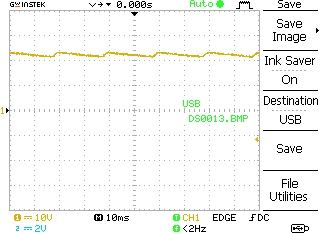
\includegraphics[width=\textwidth]{Versuch0/MesswerteVersuch2/DS0013.png}
          \caption{Ohne Stabilisierung}
    \end{subfigure}
    \hfill
    \begin{subfigure}[b]{0.45\textwidth}
        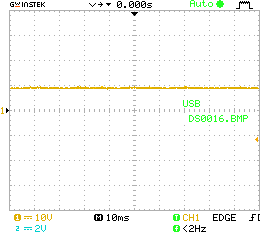
\includegraphics[width=\textwidth]{Versuch0/MesswerteVersuch2/DS0016.png}
        \caption{Mit Stabilisierung}
    \end{subfigure}


    \caption{Darstellung der Glättung und Brummspannung bei unterschiedlichen Laswiderständen.}
    \label{fig:StabBrumm}
\end{figure}

In \autoref{fig:StabBrumm} kann man den Unterschied zwischen einer Glättung und einer Glättung mit zusätzlicher Stabilisierung erkennen. Anhand der \autoref{fig:StabBrumm} und sowie der letzten Spalte \autoref{tab:Lastwiderstand_mit_Fehlern}, kann man erkennen, dass die Glättung mit zunehmender Lastwiderstand auch steigt. Dieses war zu erwarten, da die Aufladezeit des Kondensators proportional zum Widerstand ist $\tau = R \cdot C$. Bei der Stabilisierung kann man erkennen, dass diese Dazu führt, dass die Brummspannung auch geringer wird. Dieses führt zu einer stärkeren Glättung.



        \begin{thebibliography}{9}
        
        \bibitem{anleitung}
        \textit{Elektronikpraktikum -- Versuchsbeschreibungen}, Universität Bonn, 04.04.2025
        
        
        \end{thebibliography}



\end{document}